\chapter{Background}

\section{Electromagnetic Fields}
The electromagnetic fields are a collection of closely linked fields.
These fields govern the electric and magnetic interactions of charged
particles and domains. These fields can be seen in table \ref{tab:fields}

\begin{center}
    \begin{tabular}{c c c}
        \label{tab:fields}
        Field    & SI unit         & Description              \\
        \hline
        $\vb{H}$ & $1\, Am^{-1} $  & Magnetic Field           \\
        $\vb{E}$ & $1\, Vm^{-1} $  & Electric Field           \\
        $\vb{B}$ & $1\, Vsm^{-2} $ & Magnetic Flux Density    \\
        $\vb{D}$ & $1\, Asm^{-2} $ & Electric Flux Density    \\
        $\vb{J}$ & $1\, Am^{-2} $  & Electric Current Density \\
        $\rho$   & $1\, Asm^{-3} $ & Electric Charge Density
    \end{tabular}
\end{center}
These fields are described by Maxwells Equations.
In differential form for the stationary case, these are as follows:

\begin{align}
    \nabla \times \vb{H} & = \vb{J} + \frac{\partial}{\partial t}\vb{D}
    \label{eq:maxwell1}                                                 \\
    \nabla \times \vb{E} & = -\frac{\partial}{\partial t}\vb{B}
    \label{eq:maxwell2}                                                 \\
    \nabla \cdot \vb{B}  & = \vb{0}
    \label{eq:maxwell3}                                                 \\
    \nabla \cdot \vb{D}  & = \rho
    \label{:eqmaxwell4}
\end{align}
Since we're dealing with measurement of magnetic fields in this thesis,
equations \ref{eq:maxwell1} and \ref{eq:maxwell3} will naturally be of
the most interest. In simple cases, the $\vb{H}$ and $\vb{B}$ field
obey the easy relation
\begin{equation}
    \vb{B} = \mu \vb{H}
    \label{eq:BHmap}
\end{equation}
where $\mu$ is the \emph{magnetic permeability} in the domain of interest.
Formally, simple cases are where the fields are located in a medium that is
linear, homogenous across its domain, invariant depending on direction, and
stationary. Since the magnetic measurements are made inside the empty aperture
of the magnet, the domain is only made up of air. Thus, equation \ref{eq:BHmap}
holds, and the magnetic permeability is the one of free space, that is
$\mu = \mu_0 = 4\pi \times 10^{-7} Hm^{-1}$. \cite[Ch.4.1-4.4]{russenschuck2011field}


\subsection{Magnetic Flux and Induction}
Magnetic flux $\Phi$ is the total amount of $\vb{B}$ through a certain surface.
Mathematically, it is defined as:
\begin{equation}
    \Phi(\area) = \iint\limits_{\area} \vb{B} \cdot \nvec\, d\area
\end{equation}
where $\area$ is the surface, and $\nvec$ is the normal vector to the surface.
We then have the following governing laws of electromagnetism for objects at rest:
\begin{align}
    \epsilon(\partial\area) & = -\frac{d}{dt}\Phi(\area)
    \label{eq:faraday}                                   \\
    \Phi(\partial\Volume)   & = 0
    \label{eq:fluxcons}
\end{align}

\begin{figure}
    \centering
    \begin{subfigure}[b]{0.4\textwidth}
        \centering
        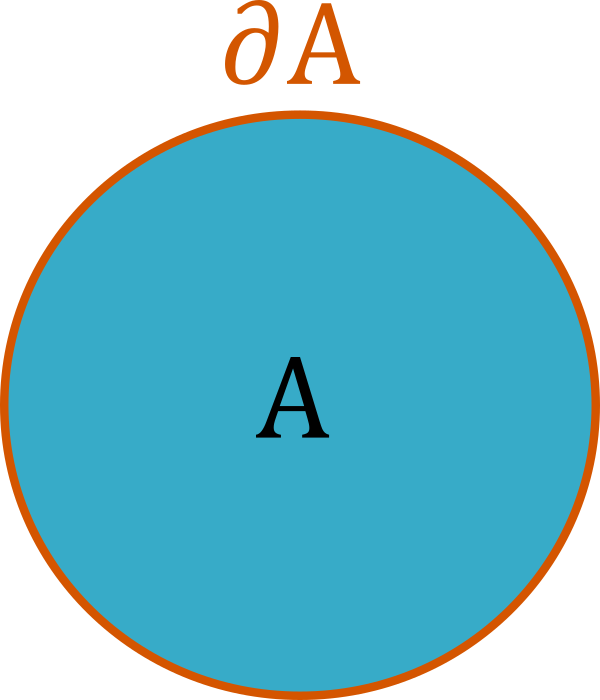
\includegraphics[width=\textwidth]{figs/partialA}
        \caption{An area $\area$ and its boundary $\partial \area$.}
        \label{fig:partialA}
    \end{subfigure}
    \hfill
    \begin{subfigure}[b]{0.4\textwidth}
        \centering
        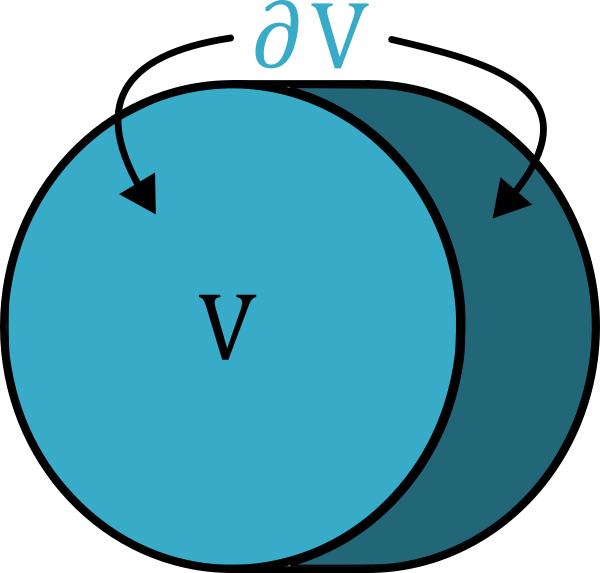
\includegraphics[width=\textwidth]{figs/partialV}
        \caption{A volume $\Volume$ and its surface boundary $\partial \Volume$.}
        \label{fig:partialV}
    \end{subfigure}
\end{figure}

Equation \ref{eq:faraday}, also called faradays law, describes the voltage\
$\epsilon$ induced in a length of wire $\partial\area$, enclosing an area
$\area$, when the magnetic flux $\Phi$ is changing with respect to time.
Equation \ref{eq:fluxcons} states that the total amount of flux flowing
through the boundary $\partial\Volume$ of the volume
$\Volume$ must equal 0. \cite[Ch.4.1.1]{russenschuck2011field}

\subsection{Series decompositions of the magnetic field}
\subsubsection{Cylindrical Coordinates}
\subsubsection{Bessel Functions}
\subsubsection{Bessel-Fourier-Fourier Series}

\section{Signal Processing}
\subsection{Filters}
\subsection{Least Squares Fitting}